\documentclass[11pt]{article}

\newcommand{\squishlist}{
   \begin{list}{$\bullet$}
    { \setlength{\itemsep}{0pt}      \setlength{\parsep}{3pt}
      \setlength{\topsep}{3pt}       \setlength{\partopsep}{0pt}
      \setlength{\leftmargin}{1.5em} \setlength{\labelwidth}{1em}
      \setlength{\labelsep}{0.5em} } }

\newcommand{\squishlistB}{
   \begin{list}{--}
    { \setlength{\itemsep}{0pt}      \setlength{\parsep}{3pt}
      \setlength{\topsep}{3pt}       \setlength{\partopsep}{0pt}
      \setlength{\leftmargin}{1.5em} \setlength{\labelwidth}{1em}
      \setlength{\labelsep}{0.5em} } }

\newcommand{\squishend}{
    \end{list}  }

\usepackage{times}
\usepackage{mathptm}
\usepackage{fullpage}
\usepackage{hyperref}
\usepackage{graphicx}

\begin{document}

\begin{center}
\medskip
{\bf{Computational Activity 3: Simulating motion of a fan cart}} 
\medskip

{\em{Derived from activity VP03 in the instructor resources that
 accompany \\ Ruth Chabay and Bruce Sherwood's {\em Matter and Interactions} 
 textbook.}}
\medskip
\end{center}

There is a typical pattern for the kinds of computational models
that you will create in this course.  The programs will generally 
follow something like this template to track the motion in small 
time steps $\Delta t$:

\squishlist
\item Define the object's initial position $\vec{r}$ and momentum $\vec{p}$.
\item Loop (forever, or until some amount of time has passed, or some
  condition has been fulfilled):
\squishlistB
  \item Calculate the net force $\vec{F}_{net}$ based on the physical 
      interactions that affect the object.
  \item Use the net force to update momentum: $\vec{p} \leftarrow \vec{p} + \vec{F}_{net} \Delta t$.
  \item Calculate velocity from momentum: $\vec{v} \leftarrow \vec{p}/m$.
  \item Use velocity to update position: $\vec{r} \leftarrow \vec{r} + \vec{v} \Delta t$.
\squishend
\squishend

\bigskip

In this activity, you will simulate the simplest nonzero net force: a constant.
For example, it might represent the force that is 
generated by a fan mounted on a cart that moves on a level track.
Here is the beginning of a VPython program that would implement that situation:

{\footnotesize{
\begin{verbatim}
from visual import *
from visual.graph import *

scene.width = 800 # pixels
scene.y = 400 # pixels

vgraph = gcurve(color=color.green)

# All dimensions are in m 
track = box(pos=vector(0,-0.05,0), length=2.0, height=0.03, width=0.10, color=color.white)
cart = box(pos=vector(0,0,0), length=0.1, height=0.06, width=0.06, color=color.cyan)

m_cart = 0.8 # kg
p_cart = m_cart * vector(0.2,0,0) # kg * m/s
delta_t = 0.01 # s
t = 0 # s
\end{verbatim}
}}

\begin{enumerate}
\item Before you run this program, please make a prediction of what will
happen: will the cart move?  Will a graph appear?  
Then, please check your prediction.
\item Modify the program to position the cart so that its left end is initially 
aligned with the left end of the track.
\item  Write a {\texttt{while}} loop to move the cart from one end of the track to the other with constant momentum.  (You did something like this in 
the previous activity.)
\item Inside the loop, instruct the computer to calculate the velocity of the cart from its mass and momentum. This will be important when we add a nonzero net force.
\item After the loop completes, print the value of the elapsed time. (Note that because of roundoff errors inherent in floating-point calculations, this value may actually be larger than the time limit you set in your {\texttt{while}} loop.)
\item Make a prediction: what should a graph of $p_x$ versus $t$ look like if momentum is constant? 
\item To fill in data points on your graph, insert the following line of code inside your loop, at the end of the loop: {\texttt{vgraph.plot(pos=(t, p\_cart.x))}}.  Was your prediction correct?
\item Add an instruction to define a constant force named {\texttt{Fnet}} (a vector) in the $+x$ direction. 
\item Add statements to the {\texttt{while}} loop in your program to update the cart's momentum to reflect the net force applied.  (See the general template above.)
\item Adjust the magnitude of the force so that it takes about half as long for the cart to reach the end of the track
with the fan turned on as it did with the fan off.
\item Explain what feature of the graph of $p_x$ versus $t$ corresponds to the constant net force applied to the system.
\item Find values for initial position, initial momentum, and net force that produce a graph of $p_x$ versus $t$ like the one below.  (You may need to let your loop run longer than before.)

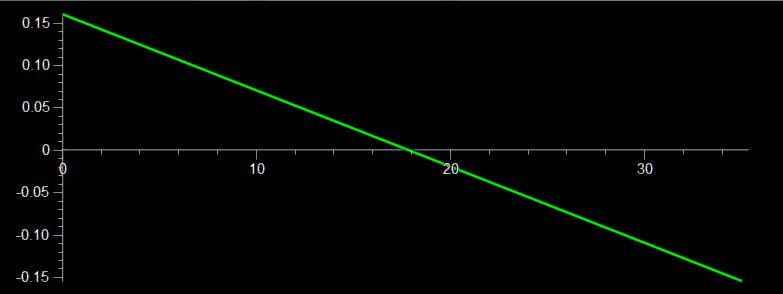
\includegraphics[width=0.9\textwidth]{px_vs_t_2.JPG}

\item Describe the motion of the cart that corresponds to this graph.

\item You're done -- please upload the final version of your program to
  WorldClass, once for each member of the group.

\end{enumerate}

\end{document}
